\section{Perancangan Block Cipher}

\subsection{Desain Blok dan Kunci}
OATSIDE menggunakan blok berukuran 64 bit sebagai konfigurasi utama, dan juga mendukung ukuran blok 96, 128, serta 192 bit. Panjang kunci utama sama dengan ukuran blok. Jumlah putaran bawaan adalah 16 dan dapat diubah melalui parameter program. Kecuali disebutkan lain, penjelasan pada bab ini menggunakan blok 64 bit.

Pada setiap putaran, blok $B$ bit dipecah menjadi enam cabang dengan urutan dari bit paling signifikan (MSB), yakni cabang luar kiri $O_L$, cabang dalam $L_1$, $L_2$, $R_1$, $R_2$, dan cabang luar kanan $O_R$. Lebar setiap cabang merupakan proporsi tetap dari $B$, seperti ditunjukkan pada tabel berikut. Cabang $L_1 \| L_2$ dan $R_1 \| R_2$ masing-masing berukuran $5B/16$ bit.

\begin{table}[H]
    \centering
    \small
    \caption{Lebar cabang (bit) untuk setiap ukuran blok}
    \label{tab:lebar_cabang}
    \begin{tabular}{@{}lcccccc@{}}
        \toprule
        \textbf{Ukuran blok} & $O_L$ ($3B/16$) & $L_1$ ($B/16$) & $L_2$ ($4B/16$) & $R_1$ ($3B/16$) & $R_2$ ($2B/16$) & $O_R$ ($3B/16$) \\
        \midrule
        64  & 12 & 4  & 16 & 12 & 8  & 12 \\
        96  & 18 & 6  & 24 & 18 & 12 & 18 \\
        128 & 24 & 8  & 32 & 24 & 16 & 24 \\
        192 & 36 & 12 & 48 & 36 & 24 & 36 \\
        \bottomrule
    \end{tabular}
\end{table}

\subsection{Struktur Putaran dan Enkripsi}
Diagram satu putaran enkripsi ditunjukkan pada Gambar \ref{fig:oatside_cipher}. Setiap putaran ke-$r$ menggunakan lima subkunci $K_1, \ldots, K_5$ yang diturunkan dari kunci putaran ke-$r$ (nanti kami bahas di Subbab \ref{subsec:key_schedule} hehe). Notasi $H_K(x)$ menyatakan fungsi SHA-256 custom kami dengan subkunci $K$ yang keluarannya dipotong ke lebar cabang tujuan, $C(\cdot)$ menyatakan kompresi 20 bit ke 12 bit, dan $S(\cdot)$ menyatakan substitusi S-box per byte.

\begin{figure}[H]
    \centering
    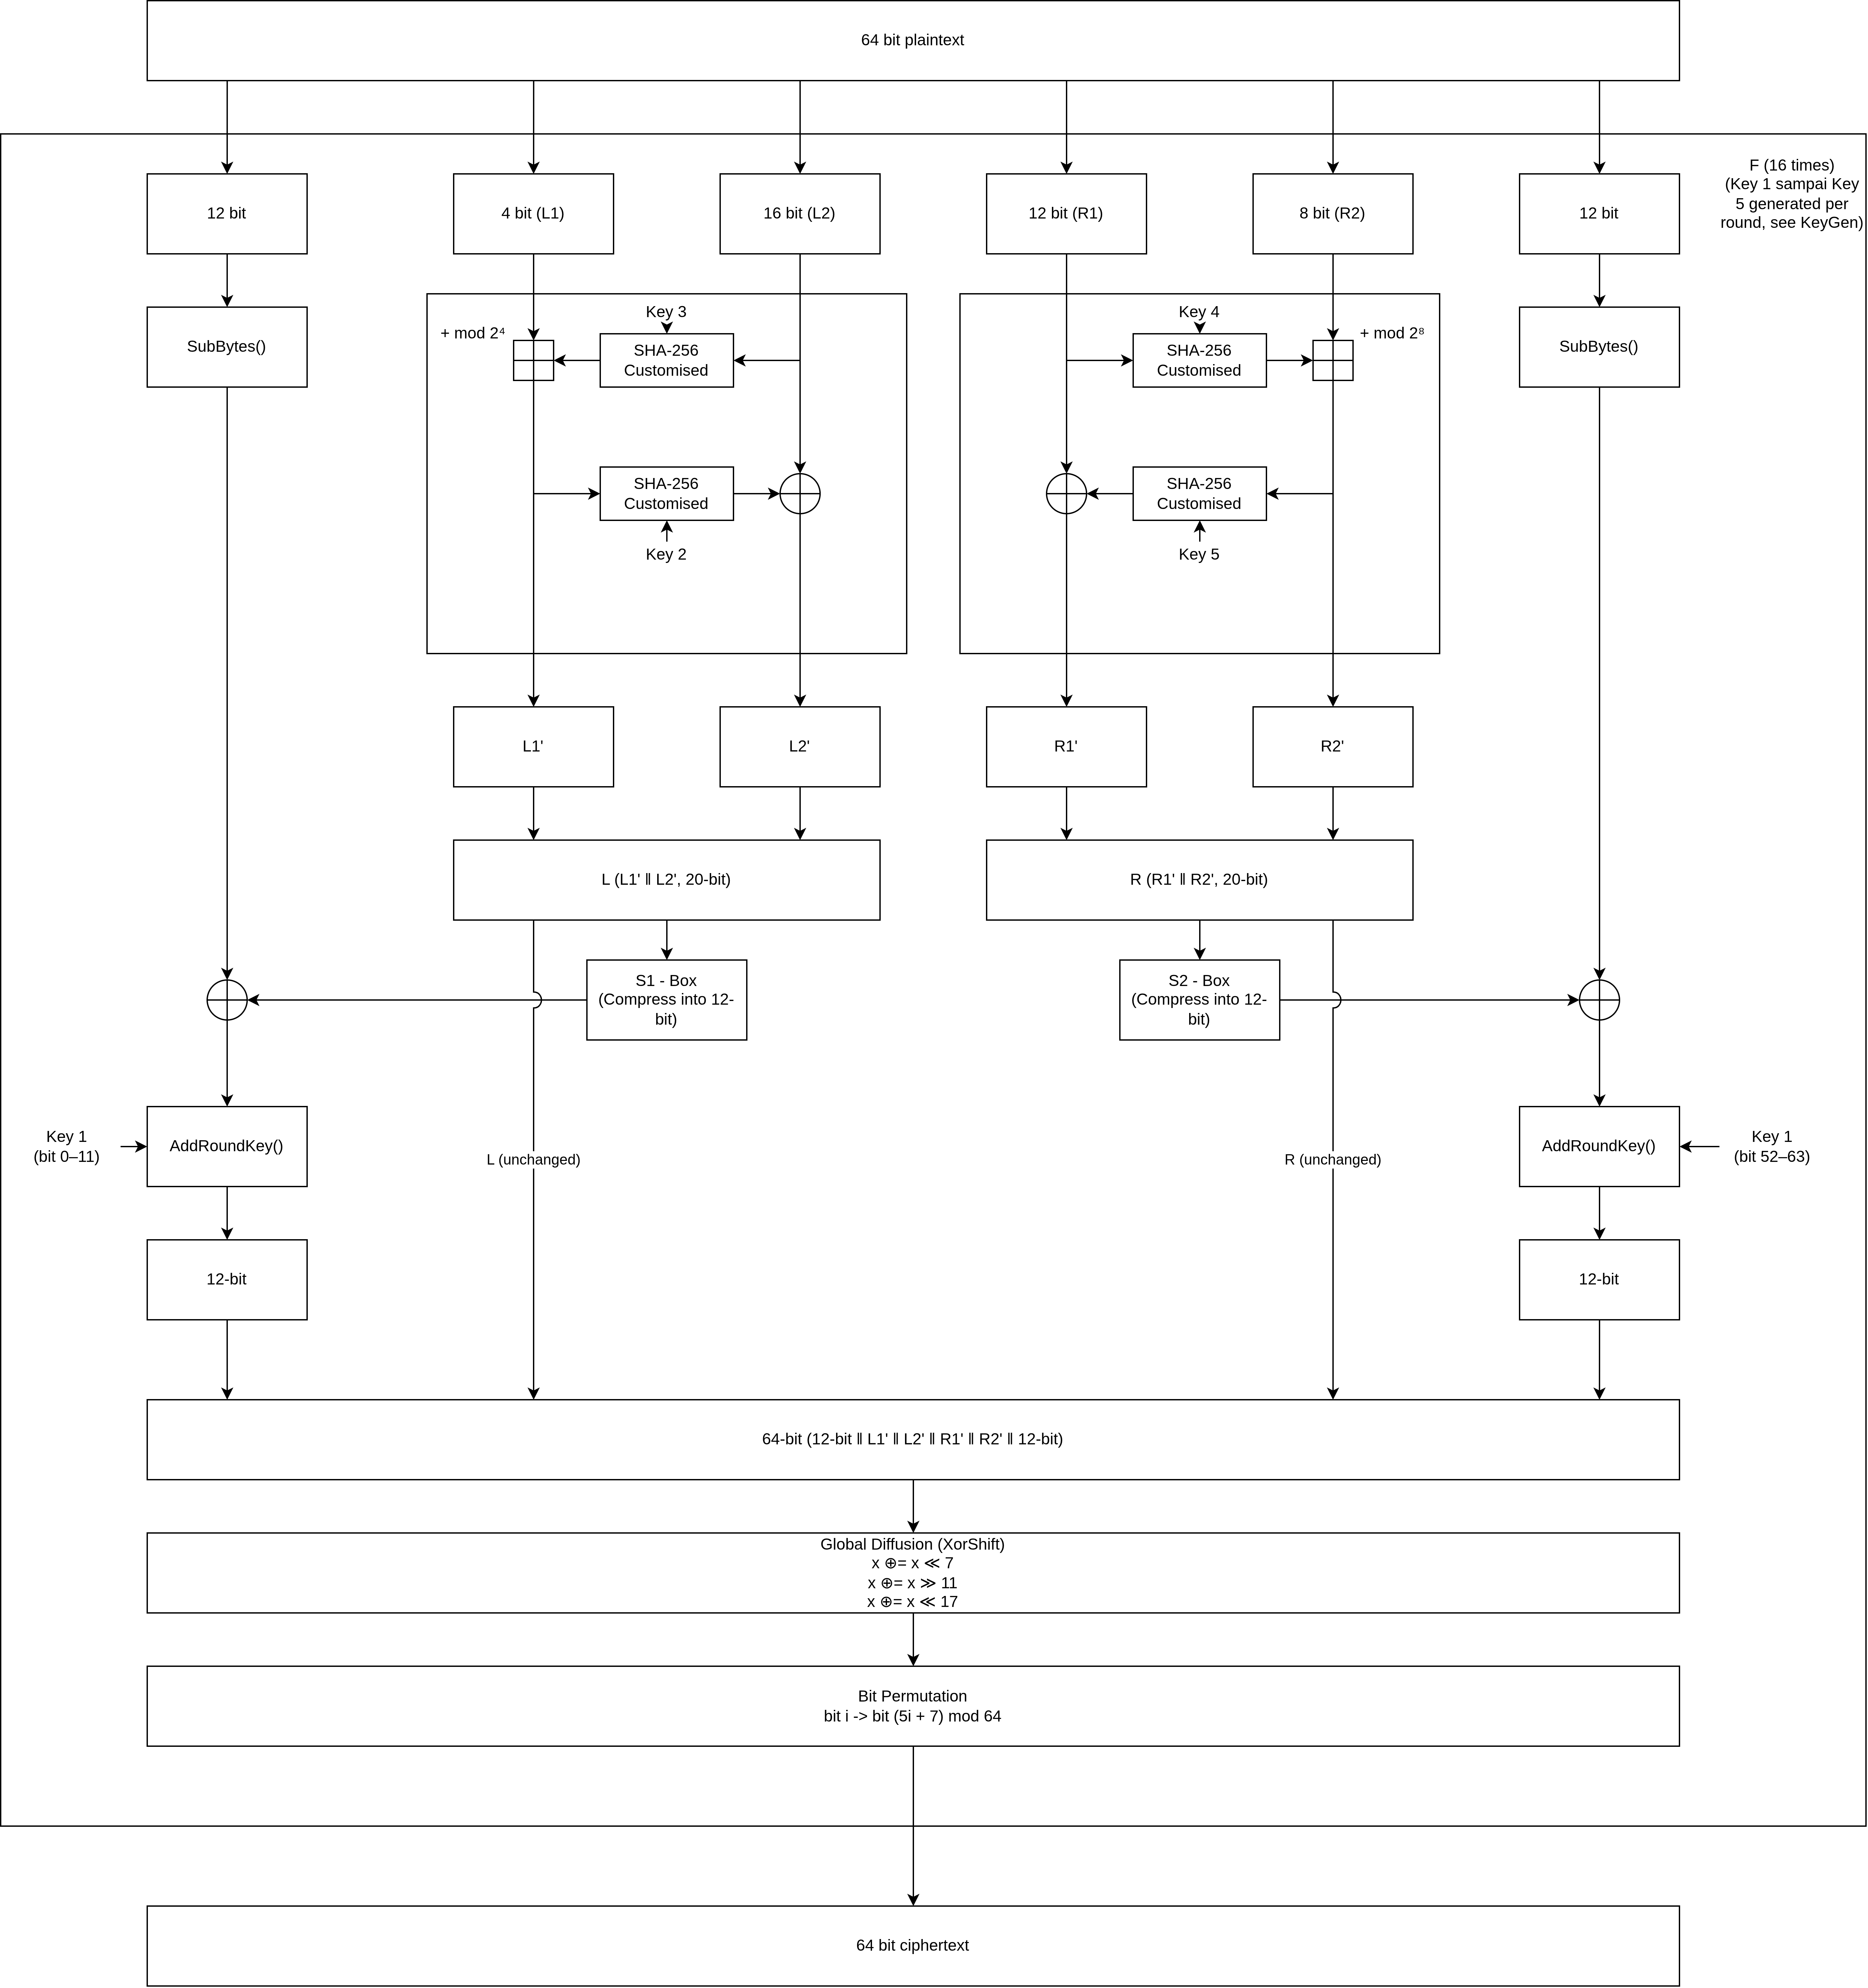
\includegraphics[width=0.85\textwidth,height=0.75\textheight,keepaspectratio]{images/oatside-cipher.png}
    \caption{Diagram satu putaran enkripsi OATSIDE (blok 64 bit)}
    \label{fig:oatside_cipher}
\end{figure}

Satu putaran terdiri atas empat tahap berikut.
\begin{enumerate}
    \item \textbf{Feistel kiri.} Pasangan $(L_1, L_2)$ diperbarui dengan
    \[ L_1' = (L_1 + H_{K_3}(L_2)) \bmod 2^{4}, \qquad L_2' = L_2 \oplus H_{K_2}(L_1'). \]
    \item \textbf{Feistel kanan.} Pasangan $(R_1, R_2)$ diperbarui dengan
    \[ R_2' = (R_2 + H_{K_4}(R_1)) \bmod 2^{8}, \qquad R_1' = R_1 \oplus H_{K_5}(R_2'). \]
    \item \textbf{Cabang luar.} Cabang luar disubstitusi, lalu di-XOR dengan hasil kompresi cabang dalam dan sebagian kunci $K_1$:
    \[ \begin{array}{l} O_L' = S(O_L) \oplus C(L_1' \| L_2') \oplus K_1[0..11], \\ O_R' = S(O_R) \oplus C(R_1' \| R_2') \oplus K_1[52..63], \end{array} \]
    dengan $K_1[a..b]$ menyatakan bit ke-$a$ sampai ke-$b$ dari $K_1$ yang dihitung dari MSB.
    \item \textbf{Difusi global dan permutasi.} Keenam cabang digabung kembali menjadi state 64 bit $x$, lalu diolah dengan tiga operasi \textit{xorshift} dan permutasi bit:
    \[ x \leftarrow x \oplus (x \ll 7), \quad x \leftarrow x \oplus (x \gg 11), \quad x \leftarrow x \oplus (x \ll 17), \]
    lalu permutasi $P$ memindahkan bit ke-$i$ ke posisi $(5i + 7) \bmod 64$.
\end{enumerate}

Enkripsi satu blok menjalankan keempat tahap di atas sebanyak jumlah putaran, kemudian state terakhir menjadi blok cipherteks. Implementasi inti juga menerima nilai \textit{whitening} awal yang di-XOR ke plainteks, tetapi seluruh mode operasi selalu mengisinya dengan nol. IV dan \textit{counter} ditangani pada tingkat mode operasi, bukan di dalam fungsi enkripsi blok.

\subsection{Komponen Algoritma}

\subsubsection{S-box}
S-box OATSIDE berukuran 8 bit dan dibangkitkan satu kali saat program dimulai. Untuk setiap byte $b$, dihitung $b^{-1}$ di $GF(2^8)$ dengan polinomial $x^8 + x^4 + x^3 + x^2 + 1$ (\texttt{0x11D}), dengan ketentuan $0^{-1} = 0$. Hasilnya dikenai transformasi \textit{affine}\footnote{kurang tahu padanan bahasa Indonesianya apa hehe.}
\[ S(b) = b^{-1} \oplus \mathrm{ROTL}_2(b^{-1}) \oplus \mathrm{ROTL}_5(b^{-1}) \oplus \texttt{0xA7}, \]
dengan $\mathrm{ROTL}_k$ menyatakan rotasi kiri sebanyak $k$ bit. Ini sebenarnya terinspirasi dari AES, tetapi polinomial, rotasi, dan konstanta \textit{affine}-nya berbeda sehingga menghasilkan tabel yang berbeda.

\begin{table}[H]
    \centering
    \scriptsize
    \setlength{\tabcolsep}{3pt}
    \caption{S-box OATSIDE}
    \label{tab:sbox}
    \begin{tabular}{@{}c|cccccccccccccccc@{}}
        & \textbf{0} & \textbf{1} & \textbf{2} & \textbf{3} & \textbf{4} & \textbf{5} & \textbf{6} & \textbf{7} & \textbf{8} & \textbf{9} & \textbf{A} & \textbf{B} & \textbf{C} & \textbf{D} & \textbf{E} & \textbf{F} \\
        \hline
        \textbf{0} & A7 & 82 & C2 & 1E & 15 & 6A & 7B & A0 & 09 & FF & B6 & 4E & C9 & F2 & 24 & B9 \\
        \textbf{1} & 07 & 52 & 7C & 95 & D8 & A6 & 53 & 94 & 67 & D9 & 0D & 35 & 91 & 5A & A8 & 60 \\
        \textbf{2} & F7 & 40 & 5D & 99 & 4A & 62 & BE & 56 & 18 & 2E & 27 & 8D & DD & 73 & 3E & BD \\
        \textbf{3} & C7 & 39 & 98 & F4 & 05 & 13 & EE & 4B & BC & 49 & AE & 9D & D7 & 1A & 44 & FD \\
        \textbf{4} & 8F & 6E & A3 & 9F & 2D & 19 & 4F & 33 & 51 & 1C & 45 & 02 & 2B & B1 & 5F & 08 \\
        \textbf{5} & 78 & 6C & 63 & 88 & 10 & 96 & B2 & 6F & 9A & 59 & 3A & 25 & 9C & 50 & AA & CB \\
        \textbf{6} & 97 & 47 & 1F & FA & CF & E8 & 0E & 76 & F6 & AD & 0A & AC & 03 & 65 & D1 & 1B \\
        \textbf{7} & 2A & 0B & D0 & 22 & D4 & CC & 4D & 14 & 68 & E3 & 79 & 85 & A1 & E4 & 7D & 37 \\
        \textbf{8} & B3 & 28 & B4 & 6D & A5 & C1 & 4C & C3 & E2 & 74 & F8 & 9B & D3 & 46 & ED & 3B \\
        \textbf{9} & DC & FC & 7A & 3C & 21 & 7E & 75 & 01 & E1 & 93 & 5B & F3 & 2C & AB & 87 & DB \\
        \textbf{A} & 48 & 7F & B5 & A2 & C5 & 36 & 30 & 16 & 8B & 17 & 3F & EC & DA & 8E & 34 & 38 \\
        \textbf{B} & CE & 69 & 2F & 0C & 9E & C0 & 11 & 43 & CD & DE & 5C & 5E & D6 & 04 & 66 & 1D \\
        \textbf{C} & BF & B0 & 20 & E0 & FB & EA & FE & 90 & 64 & 71 & 00 & DF & 84 & 80 & B8 & 32 \\
        \textbf{D} & 0F & 3D & 55 & 54 & 86 & 81 & D5 & F0 & F5 & 77 & C6 & 31 & 6B & C4 & F9 & 42 \\
        \textbf{E} & 61 & 83 & 06 & 8A & EB & E6 & 92 & AF & E9 & 8C & E5 & 57 & D2 & 26 & 89 & 29 \\
        \textbf{F} & B7 & 23 & 72 & BB & C8 & E7 & 41 & 70 & A4 & BA & F1 & A9 & CA & 58 & EF & 12 \\
    \end{tabular}
\end{table}

\subsubsection{Kompresi Cabang Dalam}
Setelah semua tahap tadi selesai, kompresi $C$ memetakan 20 bit $L_1' \| L_2'$ atau $R_1' \| R_2'$ menjadi 12 bit. Data 20 bit terlebih dahulu disubstitusi per byte, sehingga dua byte bawah melalui S-box dan 4 bit teratas diteruskan. Hasil $s$ kemudian dilipat menjadi
\[ C(v) = (s \gg 8) \oplus \big((s \bmod 2^8) \ll 3\big), \]
yaitu 12 bit teratas di-XOR dengan 8 bit terbawah yang digeser 3 posisi. 

\subsubsection{Difusi Global dan Permutasi Bit}
Di dalam satu putaran, cabang kiri dan kanan belum saling memengaruhi, dan cabang luar belum memengaruhi cabang dalam. Tahap difusi global mengatasi hal tersebut. Tiga operasi \textit{xorshift} menyebarkan setiap bit ke beberapa posisi lain, yaitu 2 sampai 8 bit keluaran untuk setiap bit masukan pada blok 64 bit. Permutasi $P$ kemudian memindahkan bit ke-$i$ (dihitung dari LSB) ke posisi $(5i + 7) \bmod B$. Karena $\gcd(5, B) = 1$ untuk seluruh ukuran blok yang didukung (permutasi ini bijektif btw).

\subsection{Penjadwalan Kunci}
\label{subsec:key_schedule}
Diagram penjadwalan kunci ditunjukkan pada Gambar \ref{fig:oatside_keygen}. Kunci putaran dibangkitkan secara berantai dari kunci utama $M$. Dengan $s_0 = M$, untuk setiap $i = 0, \ldots, n - 1$ dihitung
\[ s_{i+1} = D\big(S(\mathrm{ROTL}_{11}(s_i) \oplus RC_i)\big), \qquad RK_{i+1} = s_{i+1}, \]
dengan $D$ adalah difusi global dan permutasi bit yang sama dengan pada putaran enkripsi. Konstanta putaran $RC_i$ disusun dari byte-byte $(\texttt{0x9D} + i + \texttt{0x3D} \cdot j) \bmod 256$ untuk $j = 0, 1, \ldots$ dari MSB, sehingga setiap putaran memiliki konstanta yang berbeda.

\begin{figure}[H]
    \centering
    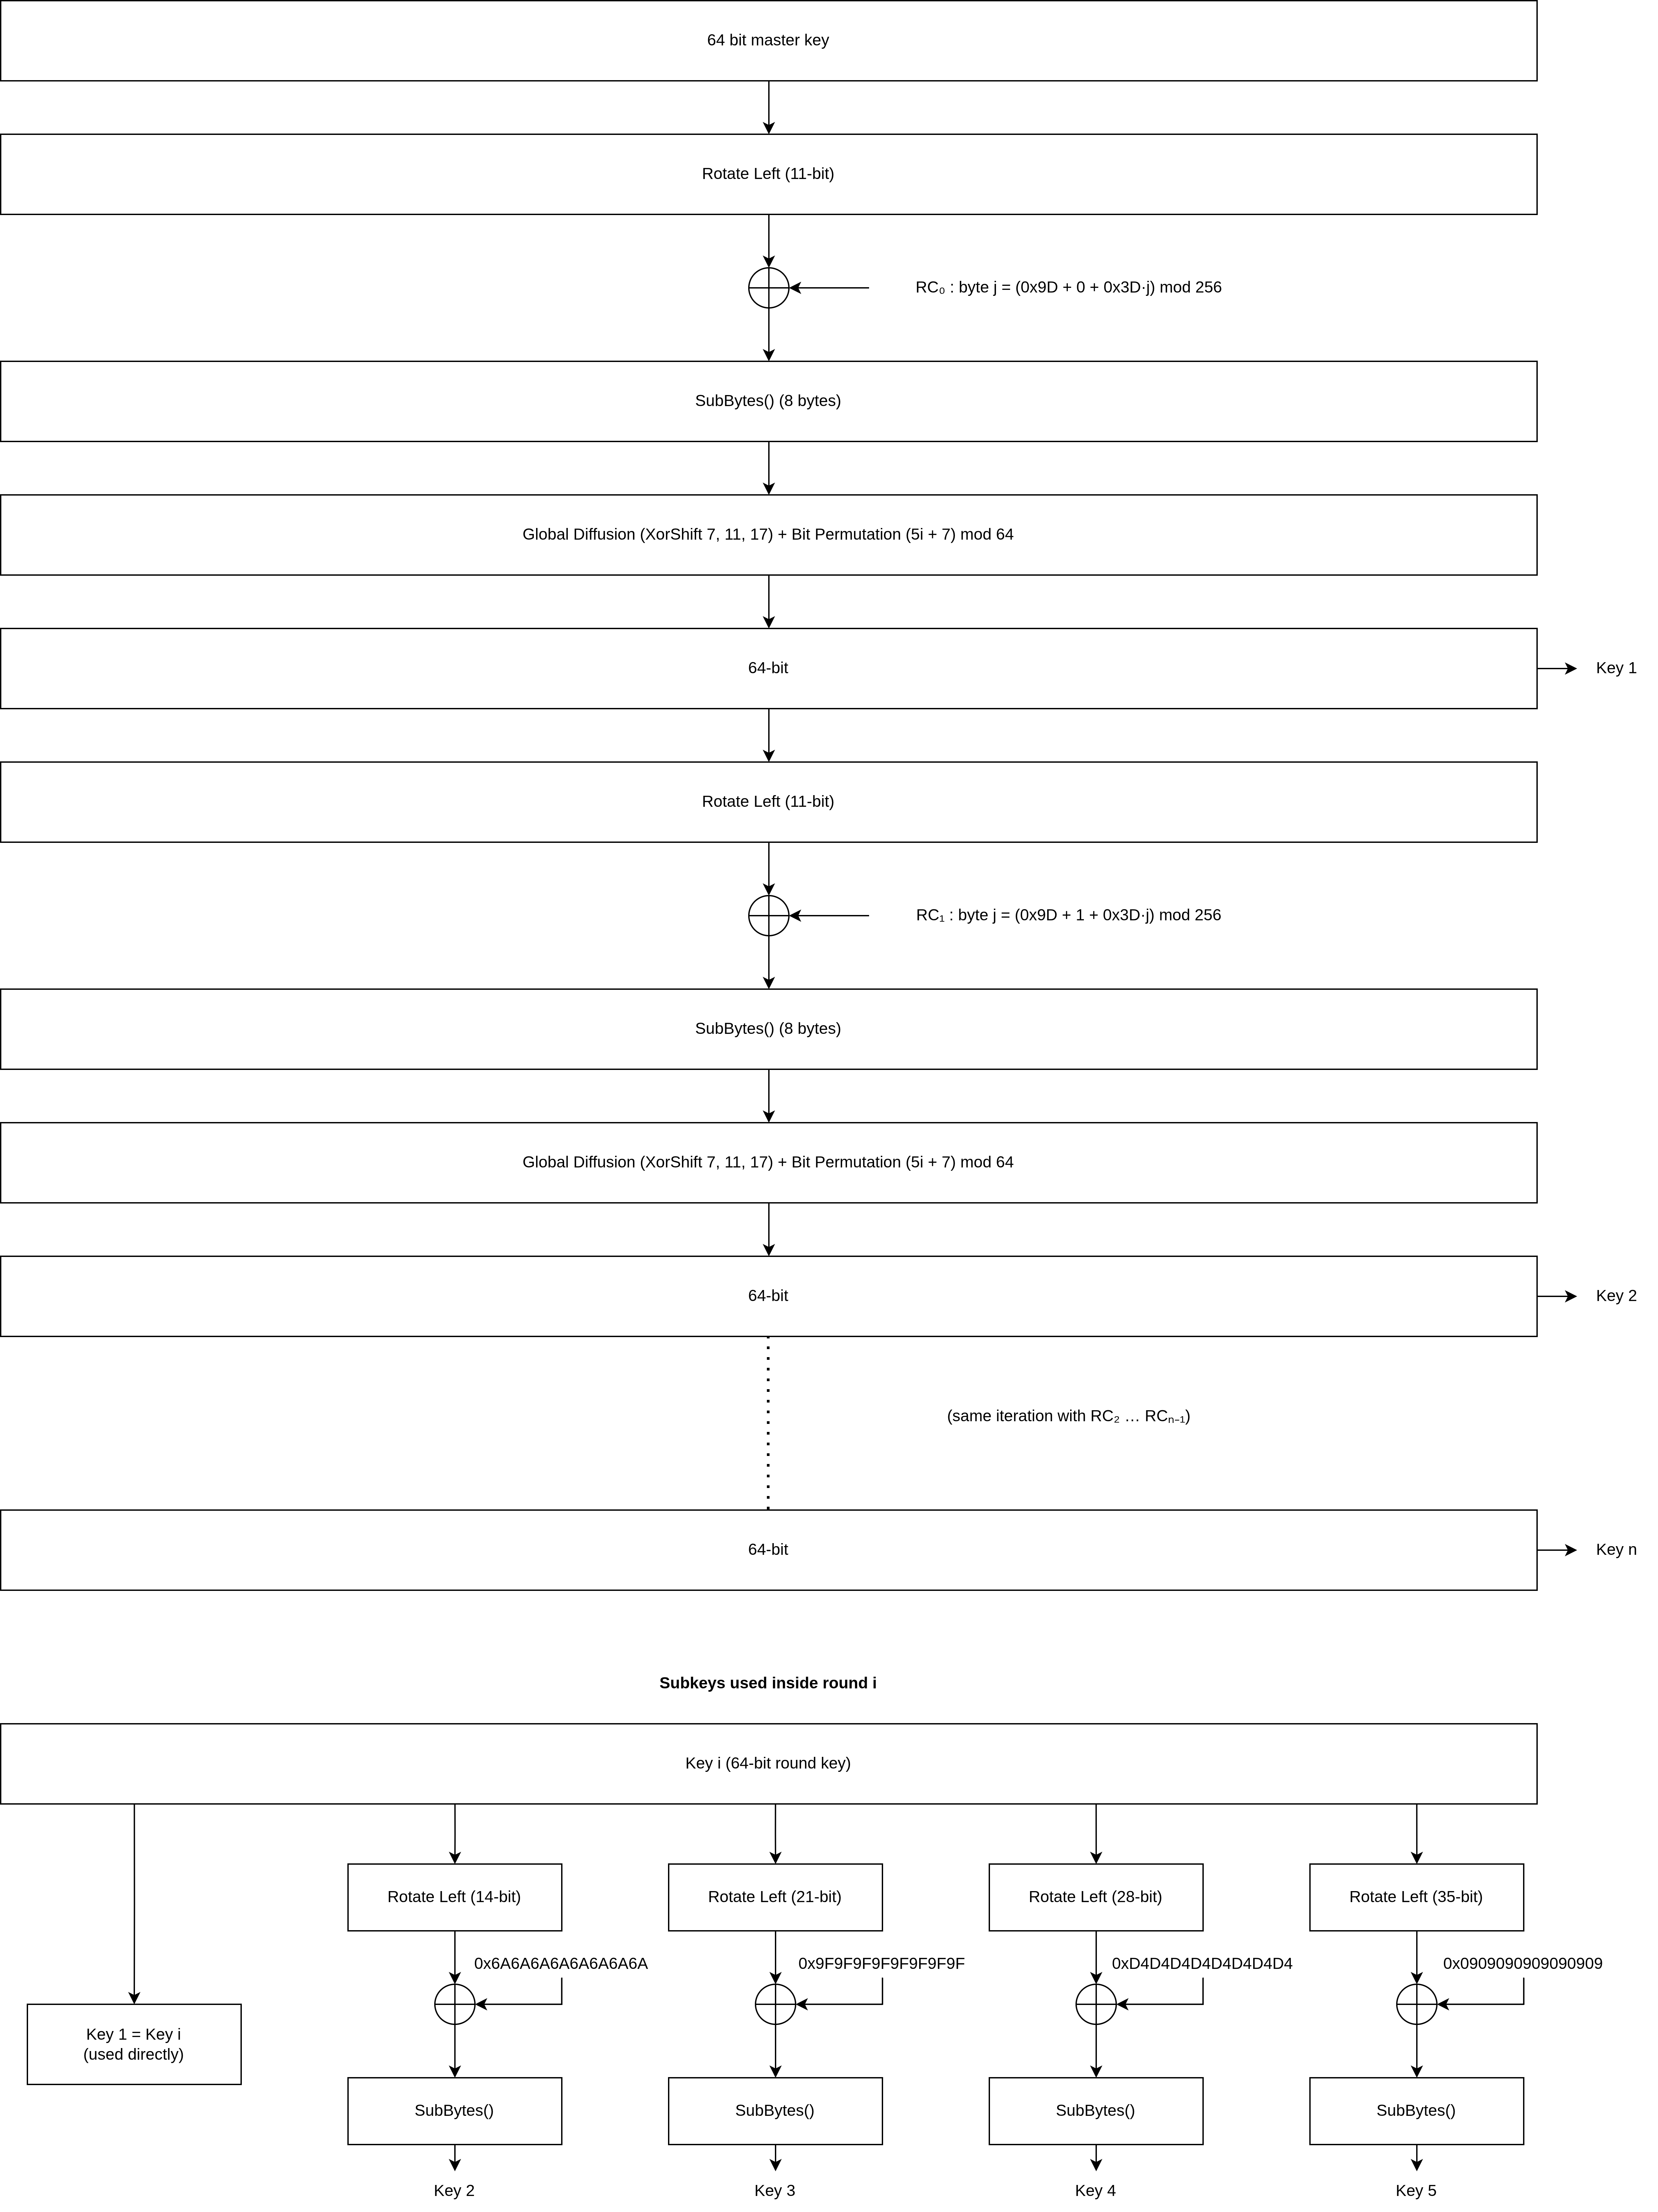
\includegraphics[width=0.75\textwidth,height=0.7\textheight,keepaspectratio]{images/oatside-keygen.png}
    \caption{Diagram penjadwalan kunci dan penurunan subkunci OATSIDE}
    \label{fig:oatside_keygen}
\end{figure}

Dari setiap kunci putaran $RK$ diturunkan lima subkunci menggunakan pemisahan domain. Subkunci $K_1$ adalah $RK$ itu sendiri, sedangkan untuk $d = 2, 3, 4, 5$ berlaku
\[ K_d = S\big(\mathrm{ROTL}_{7d}(RK) \oplus D_d\big), \]
dengan $D_d$ adalah byte $(\texttt{0x35} \cdot d) \bmod 256$ yang diulang sepanjang blok. Rincian subkunci dan pemakaiannya ditunjukkan pada Tabel \ref{tab:subkunci}.

\begin{table}[H]
    \centering
    \small
    \caption{Subkunci dalam satu putaran (blok 64 bit)}
    \label{tab:subkunci}
    \begin{tabular}{@{}cccl@{}}
        \toprule
        \textbf{Subkunci} & \textbf{Rotasi} & \textbf{Konstanta} & \textbf{Digunakan pada} \\
        \midrule
        $K_1$ & -- & -- & XOR cabang luar ($O_L$ dan $O_R$) \\
        $K_2$ & 14 & \texttt{0x6A6A\ldots6A} & $H$ kedua Feistel kiri \\
        $K_3$ & 21 & \texttt{0x9F9F\ldots9F} & $H$ pertama Feistel kiri \\
        $K_4$ & 28 & \texttt{0xD4D4\ldots D4} & $H$ pertama Feistel kanan \\
        $K_5$ & 35 & \texttt{0x0909\ldots09} & $H$ kedua Feistel kanan \\
        \bottomrule
    \end{tabular}
\end{table}

\subsection{Dekripsi}
Diagram dekripsi ditunjukkan pada Gambar \ref{fig:oatside_decipher}. \textit{Basically} proses dekripsi adalah kebalikan dari enkripsi, bahkan urutan subkuncinya juga terbalik.

\begin{figure}[H]
    \centering
    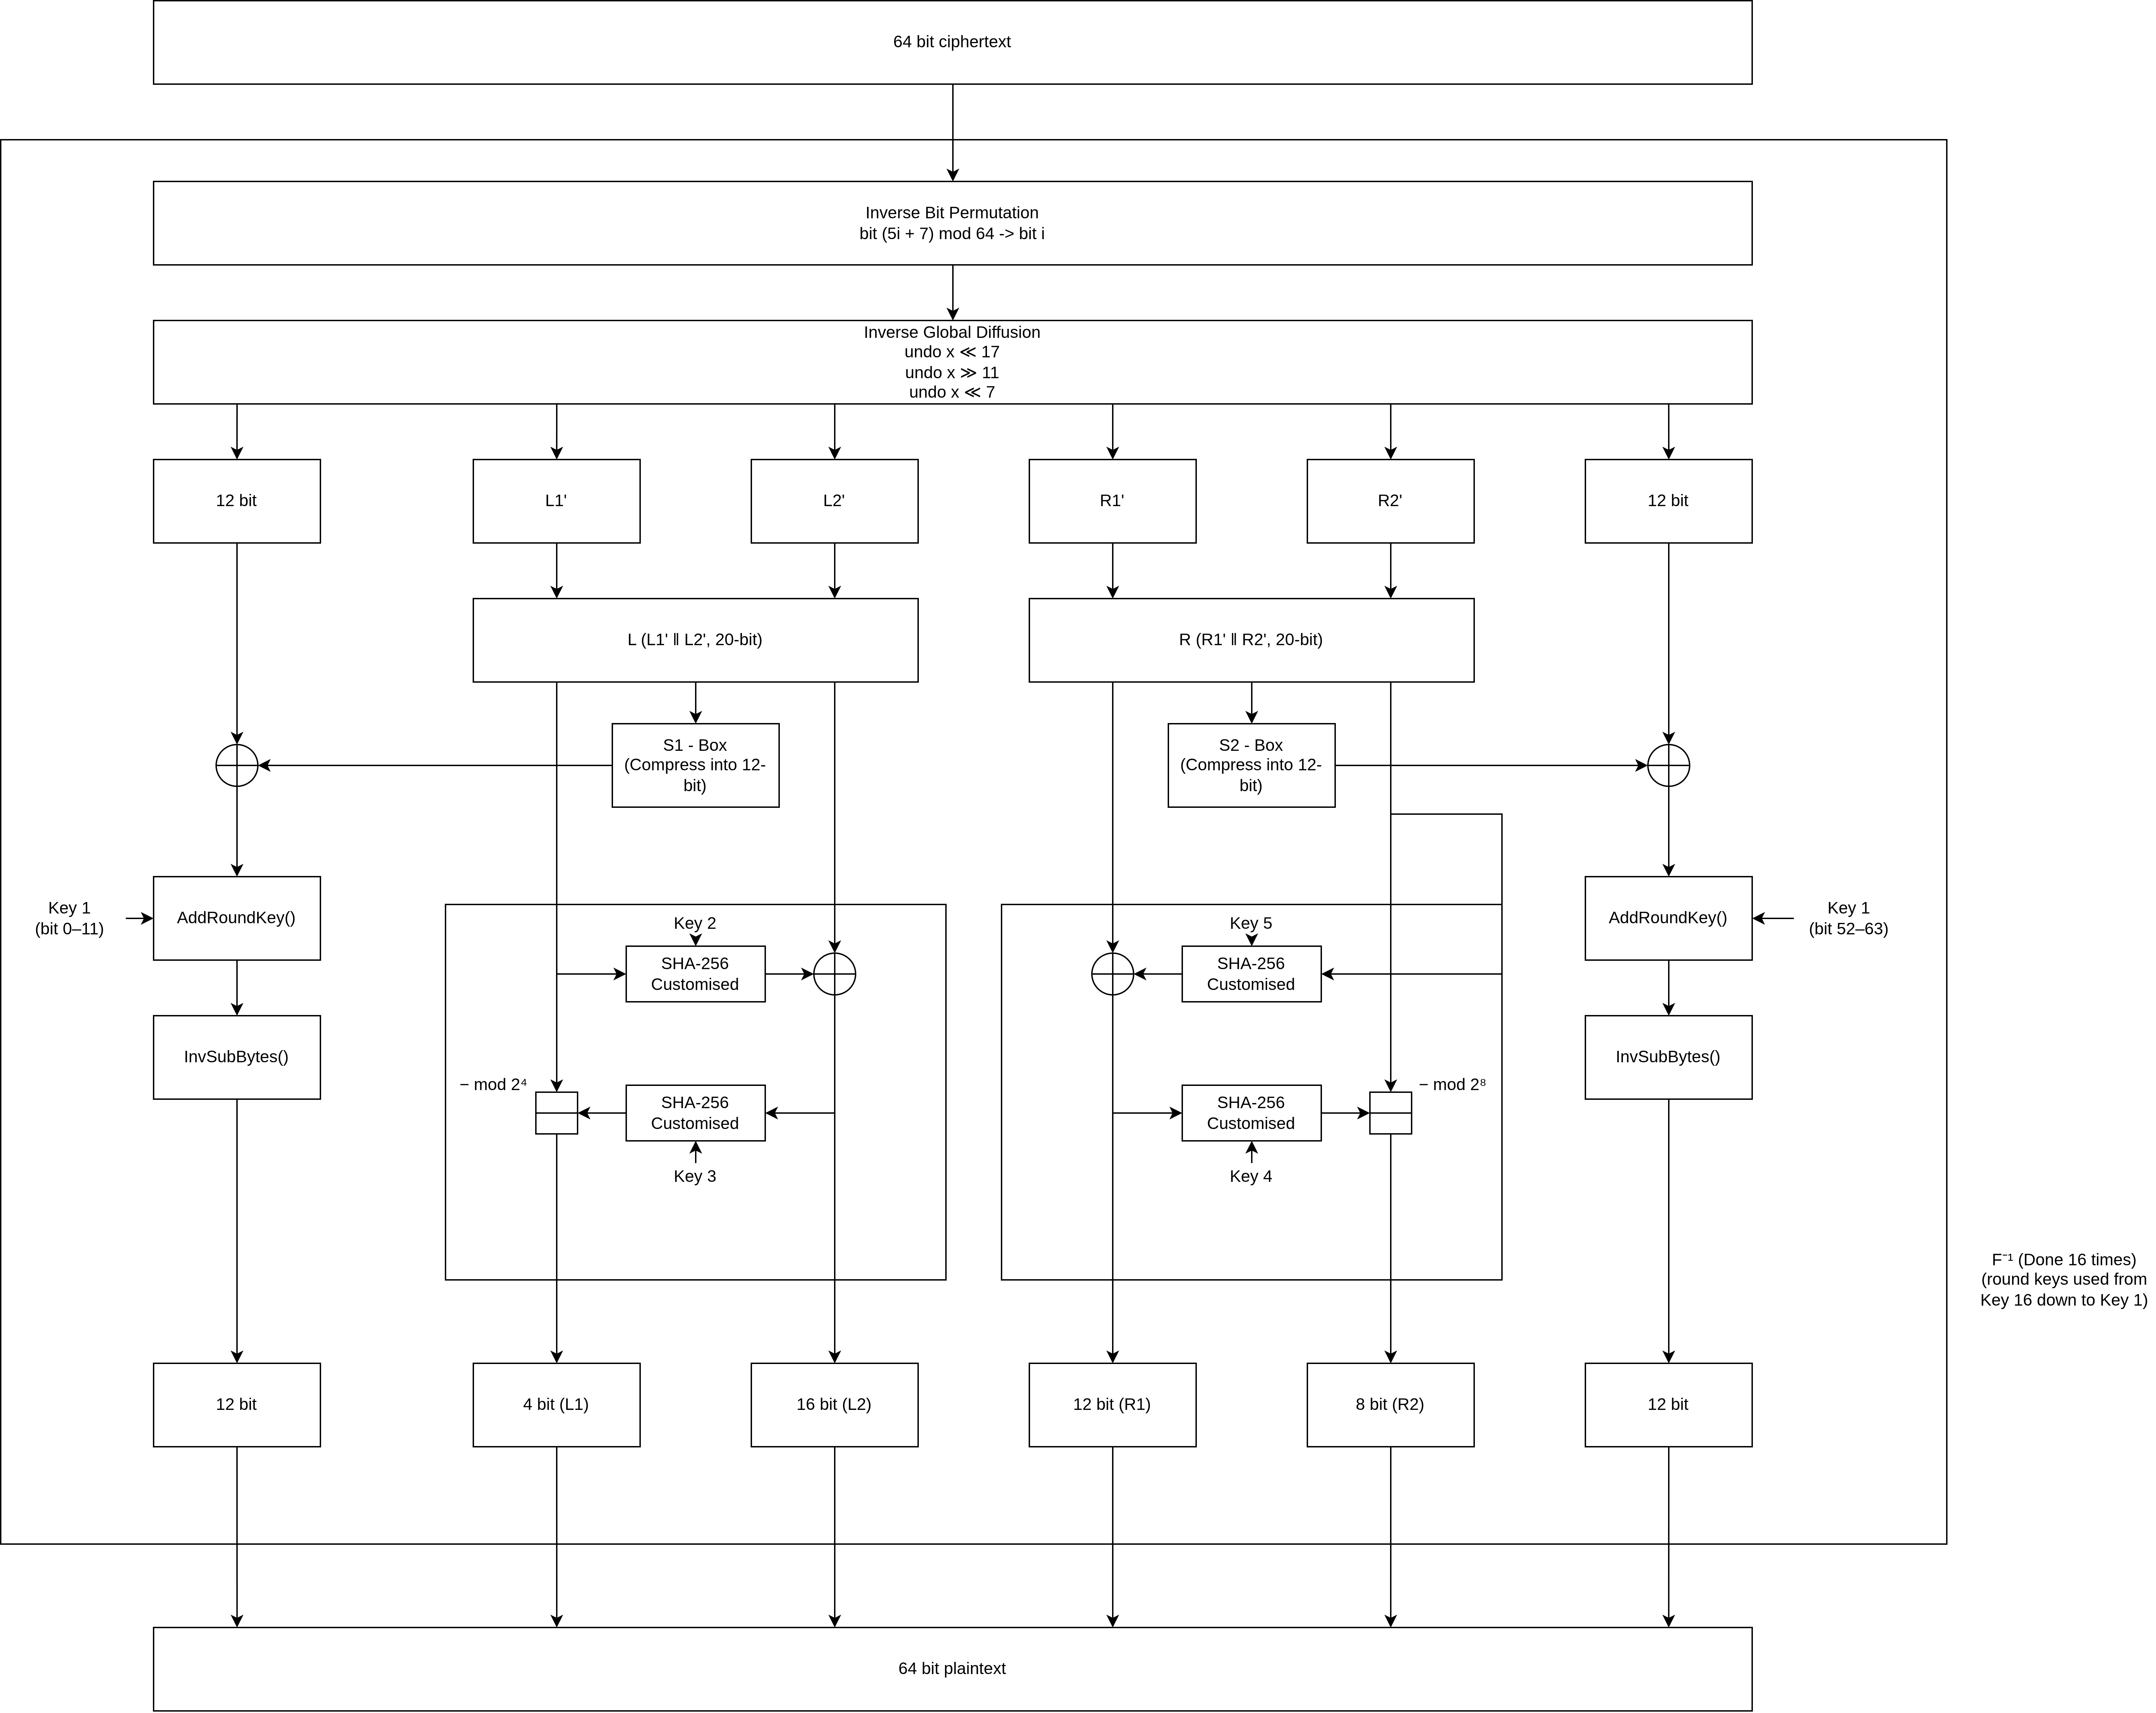
\includegraphics[width=0.85\textwidth,height=0.7\textheight,keepaspectratio]{images/oatside-decipher.png}
    \caption{Diagram satu putaran dekripsi OATSIDE (blok 64 bit)}
    \label{fig:oatside_decipher}
\end{figure}

\pagebreak
